% Since we normalized we are looking at the RATIO of reflections from different ranges.
% We REALLY should be more careful with WSS assumptions...

\chapter{Feature Extraction}

In this chapter we describe our feature extraction process. This process is an intermediary step between data preprocessing and surface classification where we calculate metrics that can be used in classification. After introducing some potential features we compare the accuracy of a few feature ensembles using a linear classifier to determine which ensemble should be used for further analysis.  

\section{Why Feature Extract?}

Machine learning algorithms fundamentally aim to extract useful patterns in data. In our case, data consist of the complex output of two radar receivers and the useful patterns we search for are patterns capable of distinguishing the surface type as either grass or non-grass. %One way to accomplish this would be to simply hand the raw \gls{iq} radar sweeps to a classifier and allow it to figure out structures in the data on its own. However, for small autonomous devices hardware capabilities are often limited and radar systems comparatively fast, making complete real-time classification of the entire bulk of acquired data cumbersome. 

We found in chapter 2 that a single radar sweep only provides information about ranges and reflectivities but cannot determine target velocities. Due in part to the normalization process done in the preprocessing step such measures alone will hardly suffice to make an efficient predictor. Instead information from a number of sequential sweeps should be used to generate a prediction. In order to make use of the information content present in the sequence of radar sweeps we have two main options. 

The first involves using a complex non linear machine learning algorithm, such as a deep neural network (\gls{dnn}) with a large number of hidden layers that figures out how to calculate efficient temporal metrics on its own. Algorithms exist that indeed can learn to analyze frequency components, for instance for speech recognition \citep{graves_mohamed_hinton_2013}, but tend to be too computationally expensive to realistically implement when hardware is limited.

Instead we utilize that we know that taking the \gls{dft} in slow time provides velocity estimates for a given distance through \gls{bf}s, as was explained in \ref{sec:doppler}. The scaling of each frequency bin thus provides an estimate of the amount of velocity component at a given range. Such estimates are rich in information regarding the topography of a surface structure, as it accounts for the \gls{rcs} of a surface at different velocities and thus different angles of incidence. 

A second option is thus to utilize this knowledge and perform \emph{feature extraction}. By extracting a smaller set of features pertaining to the frequency content of the given data, we can significantly reduce the complexity of the model. Furthermore, the feature extraction process allows us to pinpoint what data characteristics we wish to monitor, and subsequently which data characteristics we believe are of value. This ensures that the machine learning algorithm generates its predictions using patterns selected by the authors, rather than finding patterns on its own. For the reasons outlined the focus in this report is using feature extraction based machine learning. 

\section{Features}

Calculating velocity based features require the use of a sequence of multiple sweeps. How long should one such sequence be? If $T$ radar sweeps are used per classification, the rate of classifications per second, $F_c$, produced relates to the sampling rate through
\begin{equation}
	\label{eq:classification_rate}
	F_c = \frac{F_s}{T}.
\end{equation} 
Hence, the parameter $T$ becomes a tradeoff between feature accuracy and classification rate. The more samples used per classification, the better the extracted features become but with the cost of a lower classification frequency. Conversely we may be able to generate feature estimates more rapidly by setting $T$ to a lower value, but will in the process end up with worse feature estimates. 

% Described in the preceding chapter...
%The reflectivity of a material, described by its dielectric constant, shows up in the obtained IQ-demodulated sweeps in the amplitude of the returning signals. Therefore it might seem like a good idea to simply measure the energy content of a sweep and use it as a feature. However, due to inconsistencies inbetween individual sensors, sweep normalization is performed as a pre-processing step rendering such calculations unusable. We are thus left with investigating the topography of the scene. 

In this section four different types of features are discussed aimed at capturing the geometric characteristics of a target surface. From a given data matrix $x(n,t)$ consisting of $T=25$ consecutive sweeps normalized as described in section \ref{sec:norm}, we construct for each feature type a corresponding feature vector. We can then concatenate different feature vectors to form longer sets of features as we please.  

\subsection{Envelope Estimation}

First of all we may characterize a sweep by its envelope form; that is, the shape of the absolute values of the radar sweeps. We do this by simply calculating the absolute value averages in slow time to construct the estimated envelope shape $\hat{x}(n)$ through
\begin{equation}
	\hat{x}(n) = \frac{1}{T}\sum_{t=0}^{T-1}|x(n, t)|.
\end{equation}
In figure \ref{fig:sweep_average} we see what such an averaging process yields. Individual variances are suppressed to form a stable estimate of the sweep shape. With $K$ fast time samples, the estimate of the expected envelope feature vector becomes 

\begin{equation}
	\mathbf{f}_{x} = 
	\begin{bmatrix}
		\hat{x}(0) & \hat{x}(1) & ... & \hat{x}(K-1)
	\end{bmatrix}.
\end{equation}


\begin{figure}[h]
	\centering
	\includegraphics[scale=0.7]{figs_temp/features/sweep_average}
	\caption{By averaging the absolute values of a number of consecutive sweeps, we reduce noise and make samples more similar. The dashed line shows the average of the solid lines. }
	\label{fig:sweep_average}
\end{figure}


\subsection{Fourier Transform}
% "weighted velocity profile" should be used...

As discussed in section \ref{doppler} we can relate the velocity of a scatterer to its \gls{bf} through \eqref{eq:dopp}. When an entire target scene is illuminated, computing a \gls{dft} in the slow time domain thus provides a \emph{velocity profile} of the scene at every range, indicating the amount of each velocity is present for a given range. Due to the settings outlined in chapter \ref{ch:3}, no significant aliasing in the frequency spectrum should occur in theory, as the sampling rate was set with the Nyquist criterion in mind. In figure \ref{fig:fft} the \gls{dft}s of radar \gls{iq} data are shown for all surface types considered in this work. For visualization purposes the square root of the absolute values of the \gls{dft} are shown. For grass (the top two plots), it can be seen that the frequency content is contained mainly in the vicinity of the zero frequency bin, while the other materials contain considerably higher frequency components. %The \gls{rre} assumes that a scatterer is radiating isotropically. If radiation instead can be regarded to be specular in nature, the \gls{dft} provides a good measure of the surfaces topography. %[Continu. %[Continue and add a source]

%While traversing a static surface at a constant speed, one could think of it as the details on the surface, such as small rocks, are moving closer to the radar sensor. As discussed in section \ref{doppler}, this alters the frequency of the transmitted signal according to the Doppler effect, and the radar detects beat frequencies, corresponding to the frequency shifts. Depending on the surface's characteristics, the doppler frequencies may vary. 

%One way to obtain the the frequency contents is by means of the \gls{dft}. In figure \ref{fig:fft}, typical \gls{dft}s are shown for all materials. The figure is intended to show differences in the \gls{dft}s. Hence, to make the difference more clear, the squre root of the \gls{dft}s have been plotted. For grass (the top two plots), it can be seen that the frequency content is contained mainly at the zero frequency and close to it. The other materials contain slightly higher frequency content as well. Gravel, in particular, differs a lot from the other materials with a wide variety of frequency components.


% ¤¤¤¤¤¤¤¤¤¤¤¤¤¤¤¤¤¤¤¤ Comments ¤¤¤¤¤¤¤¤¤¤¤¤¤¤¤¤¤¤¤¤¤i
% is x the small or large data matrix? Here it is both...
% I think the notation looks strange here...
% Instead just write the DFT? 

%As for the feature vector, a data matrix consisting of $T$ sweeps is selected. Viewing this as a matrix with elements $x(n,t)$, we can compute a $k$-step Fourier transform for each range, $n$, and sample index $m$, as

As for the feature vector, a $T$-step DFT along the slow time axis is first computed for each range, $n$, as
\begin{equation}
	\mathbf{d}_n=\text{DFT}\big\{x(n,t)\big\}_t =  \sum_{t=0}^{T-1}x(n,t)\exp\Big(-2\pi i\frac{kt}{T}\Big), \quad k=0,...,T-1.
\end{equation}
After this, the transformations for all ranges are concatenated into a one-dimensional feature vector. This feature vector must be real-valued, as the machine learning classifiers considered in this work utilize real-valued inputs. The feature vector is formed by taking the absolute values of the frequency components through
\begin{equation}
	\textbf{f}_{f}=\begin{bmatrix} |\mathbf{d}_0|^* & |\mathbf{d}_1|^* & \hdots & |\mathbf{d}_K|^* \end{bmatrix},
\end{equation}
where $|\cdot|^*$ denotes elementwise absolute values, and $K$ is the number of fast time samples.    


% This section is weirdly written imo 
%An important remark to make is that under the assumption that the autocovariance function of a process $y_t$ decays sufficiently fast, it is closely related to the Fourier transform of the process. The Wiener-Khinchin theorem states that \citep{lu_vaswani_2009} with certain properties\footnote{The process has to be wide sense stationary. The meaning of this is defined in section \ref{ACr}.}, a process, $y_t$, the Fourier transform of its autocovariance function, denoted $\phi_y(\omega)$, relates to the Fourier transform of the actual process according to \citep{jakobsson_2015}
%\begin{equation}
%	\phi_y(\omega) = \lim\limits_{N\rightarrow\infty}E\Bigg\{\frac1N\Big|\sum^N_{t=1}y_te^{-j\omega t}\Big|^2\Bigg\}=\lim\limits_{N\rightarrow\infty}E\Big\{\frac1N|Y_N(\omega)|%^2\Big\}.
%\end{equation}
%An alternative to studying the Fourier transform could therefore be to examine the autocovariance of time series of IQ data.

\begin{figure}[h]
	\centering
	\includegraphics[scale=0.55]{figs_temp/features/fft}
	\caption{For each material, a 128-step \gls{dft} is computed in slow time for all ranges. The absolute value is taken over the complex \gls{dft}, followed by taking the square root of it to make the differences more clear in the plot. }
	\label{fig:fft}
\end{figure}


\subsection{Autocovariance in Range}
\label{ACr}

% This is actually wrong... and not well written atm
% Tie this into preceding section instead. Autocov allows for calculating the number of lags.
%An obvious surface characteristic to ponder is roughness; while a tiled surface is typically very flat, grass is characterized by a random, unpredictable structure. It is reasonable to assume that there is more correlation between two closely spaced points on the tiled surface than there is on grass. This motivates us to study the autocovariance in slow time.

A second method to investigate time-domain dependencies is through the autocovariance function. This method adds the benefit of allowing for a specification of the number of covariance lags, $q$, which can significantly reduce the number of features. Figure \ref{fig:autocorr_range} displays absolute values of autocovariances estimated from 5000 sweeps for all surface types considered. As can be observed, the tiled surface, which is the most even, corresponds to the graph with the highest autocovariances. In contrast, the arguably most uneven surface - grass - is represented by the graph with the lowest autocovariances.

\begin{figure}[h]
	\centering
	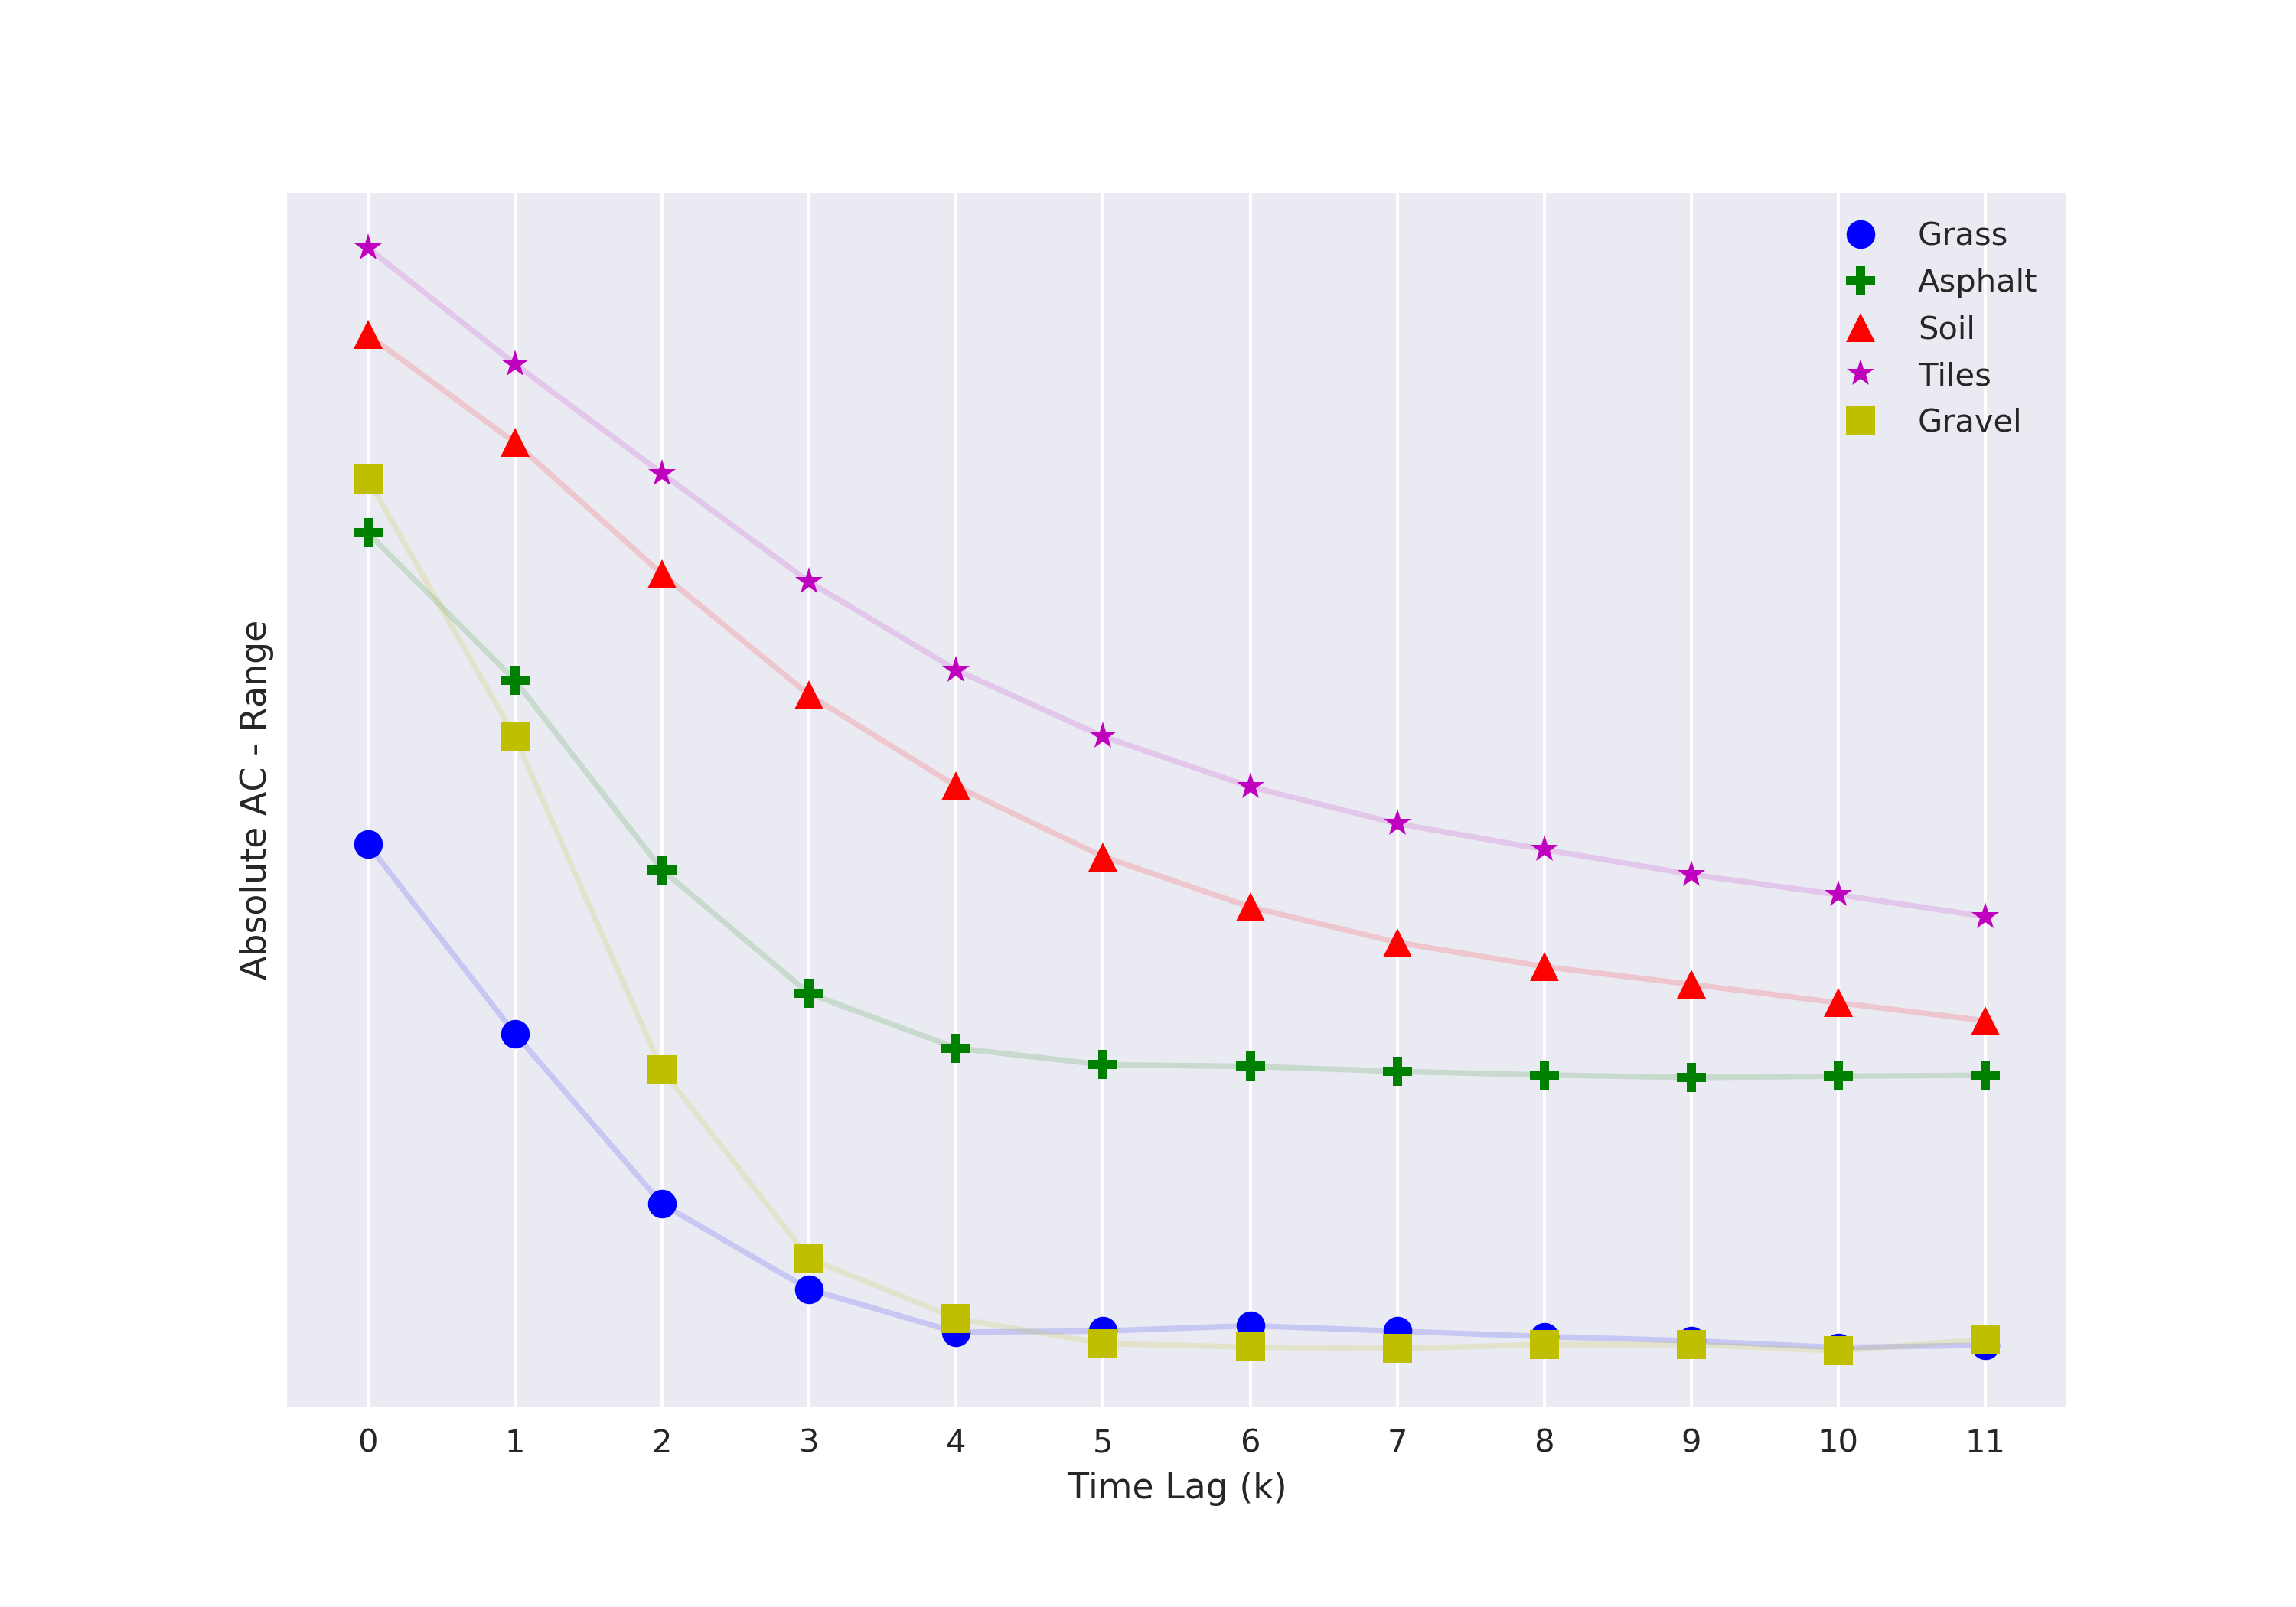
\includegraphics[scale=0.45]{figs_temp/features/autocorr_range.png}
	\caption{The graphs show the absolute values of the autocovariances computed from a time-varying \gls{iq}-signal recorded at a range of approximately 14 cm.}
	\label{fig:autocorr_range}
\end{figure}

%We can regard the sequence $\{x(n,t)\}_{t=t_m}^{t_m+T-1}$ of measurements of range $n$ as samples from a stochastic process $X_{n,t}$ with the autocovariance function

%\begin{equation}
%	C_{XX}(n,t,s) = \text{Cov}(X_{n,t},X_{n,s}).
%\end{equation}


% We should maybe remove this tbh... or at the very least move it
%\noindent
%If we then can consider the process to have the following three properties:
%\emph{
%\begin{enumerate}
%	\item Constant finite mean
%	\item Autocovariance function only dependant on the difference $(s-t)$ and not on actual values of $s$ and $t$.
%	\item Finite variance
%\end{enumerate}
%}
%\noindent
%over the time interval $t_m$ to $t_m+T-1$, it can be regarded as a \emph{Wide-Sense Stationary} (WSS) process \citep{jakobsson_2015}. The first and second assumptions require the returning signal to carry some level of stability, which is reasonble considering the short time-frame $T/F_s$ considered. 


%We assume that $x(n,t)$ are samples from a stochastic process $X_{n,t}$ which is wide sense stationary (WSS) \citep{jakobsson_2015} over some short time $T/F_s$. Its autocovariance function for some range, $n$ may then be defined as
%\begin{equation}
%	r_n(k) = {\E}_t\big\{(X_{n,t} - \mu_n)^*(X_{n,t+k} - \mu_n)\big\}
%\end{equation}
%where $\mu_n=\E_t\{X_{n,t}\}$. We can form the (biased) estimate of the autocovariance function through

For practical reasons, only $T$ sweeps are used for estimates in the model. The biased estimate of the autocovariance function can be obtained through \citep{jakobsson_2015}
\begin{equation}
\label{eq:ac}
	\hat{r}_n(k) = \frac{1}{T}\sum_{t=k}^{T-1}\big(x(n,t) - \hat{\mu}_n\big)\big(x(n,t-k) - \hat{\mu}_n\big)^*
\end{equation}
where 
\begin{equation}
	\hat{\mu}_n = \frac1T \sum_{t=0}^{T-1}x(n,t).
\end{equation}

The bias in this estimate is completely inconsequential as all features later are normalized to zero mean unit variance. Estimating the autocovariances through \eqref{eq:ac} does assume that $x(n,t)$ is wide sense stationary, but for a rough real world terrain, this assumption is optimistic. However, the estimates may nonetheless make for useful metrics for classification as they feature temporal changes. The features may be formed as
\begin{equation}
	\hat{\mathbf{r}}_{k} = 
	\begin{bmatrix}
		\hat{r}_0(k) & \hat{r}_1(k) & ... & \hat{r}_{K-1}(k)
	\end{bmatrix}.
\end{equation}

Noting that the autocovariance sequence at 0 lag produces only real numbers, as any complex number $z = a + bi$ multiplied with its conjugate has zero imaginary part $\text{Im}(zz^*) = \text{Im}((a + bi)(a - bi)) = \text{Im}(a^2 + b^2) = 0$, we may form the full real-valued feature component for $q$ autocovariance lags $\mathbf{f}_{r}$ as
\begin{equation}
	\mathbf{f}_{r} = 
	\begin{bmatrix}
		\hat{\mathbf{r}}_{0}  & \text{Re}(\hat{\mathbf{r}}_{1} ) & \text{Im}(\hat{\mathbf{r}}_{1} ) & ... & \text{Re}(\hat{\mathbf{r}}_{q} ) & \text{Im}(\hat{\mathbf{r}}_{q} )
	\end{bmatrix}.
\end{equation}


%%%%% DISCUSSION OF AUTOCOV/CORR IMAGE %%%%%
%From figure \ref{fig:autocorr_range}, we see that the the 1-step autocorrelation is what separates grass from other materials the most. For the feature vector we choose $q=2$, thus ncluding the variance as well as autocovariance steps 1 and 2 for the normalized sweeps.

%Figure \ref{fig:autocorr_range} illustrates the normalized autocorrelations for the different materials at a certain range. As expected, grass and tiles are two extremes in terms of roughness, and the other materials lie somewhere inbetween. Below, we explain how the autocovariance is formed in terms of features as preparation for the classifier.


\subsection{Autocovariance in Energy}

While the sweep normalization process rendered absolute mesurements of signal energy meaningless, we are still able to investigate its time-dependant structure through the autocovariane function. First we estimate the energy in each radar sweep $v(t)$ and the average energy $v_a(t)$ in $T$ number of sweeps, and then calculate the real-valued autocovariance sequence $h(k)$ as 

\begin{equation}
	v(t) = \frac{1}{N}\sum_{n=0}^{N-1}x(n,t)x^*(n,t)
\end{equation}

\begin{equation} 
	v_a = \frac{1}{T}\sum_{t=0}^{T-1}v(t)
\end{equation}

\begin{equation}
	h(k) = \frac{1}{T}\sum_{t=k}^{T-1}\big(v(t) - v_a\big)\big(v(t-k) - v_a\big)^*.
\end{equation}

As $h(k)$ only consist of real values, the energy autocovariance feature vector $\mathbf{f}_{h}$ is formed as

\begin{equation}
	\mathbf{f}_{h} = 
	\begin{bmatrix}
		h(0) & h(1) & ... & h(q-1)
	\end{bmatrix},
\end{equation}
where $q$ is the number of covariance lags. 

%We can also calculate the autocovariance function of estimated sweep energy. Although the sweeps are normalized in the preprocessing, we can investigate how the sweeps change over time. 

%The average energy in a sweep tells us how much energy is reflected back to the radar. Hence it can be regarded as a measure of how good of a reflector the underlying surface is. The energy depends on the shape of the surface, as well as its dielectric constant. Compared to other materials, grass has a very different surface shape, which potentially gives it a very different reflexivity. However, its dielectric constant could also vary a lot depending on whether it is wet or dry, making it hard to guess its reflective properties.

%By computing the average energy of single sweeps from different surfaces we see in figure \ref{fig:sweep_energy} that grass reflects much less energy. This indicates that the average sweep energy is a good feature for binary grass/not grass classification. However, in order to get a more robust measure of the average energy we do not only compute the average over selected range bins of a single sweep, but we average over a few consecutive sweeps as well. Mathematically, the feature we end up using becomes
%\begin{equation}
%	P(t_m) = \frac{1}{NT}\sum_{t=0}^{T-1}\sum_{n=0}^{K-1}x(n, t_m + t)x^*(n, t_m + t),
%\end{equation}
%where (describe variables)

%Despite the fact that the average energy appears to be a highly relevant feature, it is also much gain dependent, and conflicts with what is stated in section *reference to sweep norm.*. Therefore, if different sensors are to be used for training and future classifications, this feature will not be of any use.


\begin{table}
\rowcolors{2}{gray!25}{white}
\begin{center}
  \begin{tabular}{|c|cccccc|}
\hline
    \rowcolor{gray!150}
		  & \color{white}\textbf{Abs} & \color{white}\textbf{AC Energy} & \color{white}\textbf{AC Range} & \color{white}\textbf{FFT} & \color{white}\textbf{Features} & \color{white}\textbf{SVM Accuracy} \\
	  Config 1 & X &   &   &   & 28  & 92.23 \\
	  Config 2 & X & X & X & & 174 & 97.44 \\
	  Config 3 & & & & X & 700 & 97.37 \\
\hline
  \end{tabular}
\end{center}
\caption{Three possible configurations of feature. Ideally, we want few features and a high accuracy.}
\label{tab:feat}
\end{table}


% "The same model" is the hyperparameter optimized model we later get to, so the ordering is strange here. Numbers are off too.

\subsection{Reducing the Range Swath}

Before performing any feature processing, the data is downsampled by a downsampling factor of $D=20$ as was described in section \ref{downsampling}. However, after examining the fast time samples it turns out that ranges below approximately 11 cm only contain little information. This can clearly be seen in the dark regions of the \gls{dft}s in figure \ref{fig:fft}. Similarly, yet not as apparent, little information is found at longer ranges. Therefore we extract samples from an intermediate region when downsampling, modifying equation \eqref{eq:downsamp} to become
\begin{equation}
	r_{1,D}(d, t) = r_{1}(50+dD,t), 
	\quad \text{and} \quad r_{2,D}(d,t) = r_{2}(50+dD,t)
\end{equation}
for $d=0,...,13$. With this definition, the downsampled signal consists of 14 evenly spaced range indices from 50 to 310, corresponding to ranges 9.4 to 21.88 cm. Thus, the resulting data matrix used for generating one set of features has $14\times 2$ ranges for the two sensors and has $T=25$ slow time sweeps. 

\subsection{Tested Feature Combinations}

Four different feature extraction methods have now been described - the average signal shape, the autocovariance in range and energy as well as the Fourier transform. The methods each generate a number of features. However, we are not limited to feed our model with features taken from a single one of the methods. In table \ref{tab:feat}, three possible configurations of features are chosen. Each of these combinations was tested in a simple support vector machine classifier (\gls{svm}, described in further detail in chapter 5), to evaluate which was the most efficient. The first one, which simply involves the averaged sweep envelope, requires much fewer features than the other two combinations - 28 positive real numbers for the 28 ranges. But looking at its performance, these features are not enough to reach the accuracy attained in the other two cases. 

By instead selecting autocovariances with 3 lags as features the accuracy increases by nearly 5 percent. Here we also include the absolute values as features, as this information is lost when subtracting the mean during the computation of the autocovariances. This configuration generates a feature vector with 174 elements, as seen in figure \ref{fig:feat_fig}. 28 features come from the absolute values and 6 from the energy autocovariance. The majority of the features come from the autocovariance in range. For each of the 28 range bins there is one real-valued feature representing variance followed by two complex autocovariances for each range bin. This should give us $28+2\cdot 28=84$ features, but as the real- and imaginary parts of complex numbers are split up in two features, we obtain $28+2\cdot2\cdot 28=140$ features. The total number of features therefore becomes $28+6+140=174$.

\begin{figure}[h]
	\centering
	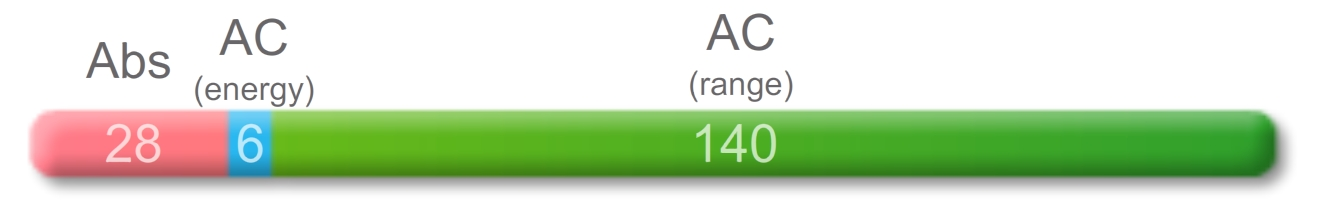
\includegraphics[scale=0.8]{figs_temp/features.jpg}
	\caption{Origin of the 174 features in features in feature configuration 2.}
	\label{fig:feat_fig}
\end{figure}

We can also choose to look at the Fourier transform, as in configuration 3. Using the \gls{dft} we reach a similar accuracy as in configuration 2 but require some 700 features. The 700 features is a result of computing a discrete Fourier transform along the slow time of all 28 ranges over 25 samples\footnote{Ideally, the \gls{dft} should be computed as an FFT over a number of slow time samples which is a power of 2. However, to get a fair comparison of the feature extraction methods, we utilize the same number of samples for all methods.}. The length of each transform is 25, and by concatenating them all into one feature vector, we end up with $28\cdot 25=700$ elements. 

The high accuracy and low number of features of configuration 2 makes it the clear top performer of the three, and will be used for the remainder of this report for further investigation.

\section{Feature Principal Component Analysis}

Through the feature extraction methods described in previous sections we obtain high dimensional feature vectors. Getting an intuitive feel for such data extracted in these processes is difficult as direct plotting is limited to three dimensions. 

\gls{pca} is  a classical technique in statistical data analysis which takes a large set variables from a multivariate dataset and finds a smaller set of variables with less redundancy. Critically, \gls{pca} finds a rotated orthogonal coordinate system such that the elements of the set become uncorrelated \citep{hyvasrinen_karhunen_oja_2004}. Projecting elements onto the principal axes corresponding to the directions of maximal variance a good approximation of the original data in lower dimension is obtained.

After having chosen to proceed with feature configuration 2 in table \ref{tab:feat}, the 174 dimensions can be reduced to 2 dimensions using \gls{pca}. By projecting feature vectors onto the two directions of maximal variance, we get a good visualization of the separability of the different surfaces as seen in figure \ref{fig:pca}. Note that each dot in thie plot corresponds to one feature vector, and that the figure represents features extracted from the full set of 175 minutes of data.  

\begin{figure}[h]
	\centering
	\includegraphics[scale=0.50]{figs_temp/pca_analysis.png}
	\caption{By performing a principal component analysis on the feature vectors we project 174 dimensional feature vecors into two dimensions corresponding to directions of maximum variance. This allows for us to visualize how separable the different surface types are.}
	\label{fig:pca}
\end{figure}

